\documentclass[MTech]{iitmdiss}
\usepackage{times}
\usepackage{t1enc}
\usepackage{graphicx}
%\usepackage[hypertex]{hyperref}
\usepackage{amsmath} 
\usepackage{multicol}
\usepackage{algpseudocode}
\usepackage{fancyhdr}
\usepackage{algorithm}
\usepackage{array, booktabs, caption}
\usepackage{ragged2e}
\usepackage{algpseudocode}
\usepackage{algorithm}
\usepackage[algo2e]{algorithm2e}
\usepackage{algorithmic}
\usepackage{natbib}
\usepackage{bibunits}
%\newcommand{\Rmnum}[1]{\expandafter\@slowromancap\romannumeral #1@}
\usepackage{etoolbox}
\documentclass{book}
\usepackage[toc,page]{appendix}
\usepackage[titletoc]{appendix}
\begin{document}
\nocite{*}
\setcounter{equation}{1}

%%%%%%%%%%%%%%%%%%%%%%%%%%%%%%%%%%%%%%%%%%%%%%%%%%%%%%%%%%%%%%%%%%%%%%
% Title page

\title{	
ANALYSIS OF MOBILE SINK BASED BIG DATA GATHERING IN DYNAMIC WIRELESS SENSOR NETWORKS}
\regno{207353}
\author{ANTU RAJ S}
\guide{SANGEETHA JOSE}
\pos{Assistant Professor}

\date{JANUARY 2016}
\department{INFORMATION TECHNOLOGY}

\maketitle

\certificate
\vspace*{0.2in}
\noindent 
 \textit{Certified that the Mini Project report entitled
} \textbf{"Analysis of Mobile Sink Based Big Data Gathering in Dynamic Wireless Sensor Networks
"} \textit{, is a bonafide work done by} \textbf{Ms. ANTU RAJ S (Reg No:207353)}\textit{ in partial fulfilment of the award of the Degree of Master of Technology in Information Technology (Specialization:Network Engineering) from Mahatma Gandhi University, Kottayam, Kerala during the academic year 2015-16.}
\\ \\ \\ \\
\vspace*{1.2in}
\hspace{.25in}
\begin{minipage}{0.18\textwidth}
\centerline{\bf Prof. K R Remesh Babu} 
\centerline{HoD$\& $ Project Coordinator} 
\end{minipage}
\begin{minipage}{.5\textwidth}
\hspace{0.15\textwidth}
\end{minipage}
\begin{minipage}{0.18\textwidth}
\centerline{\bf Dr. Sangeetha Jose} 
\centerline{Guide$\&$ Project Coordinator} 
\end{minipage}
\newline
\vspace{.15in}
\hspace{.25in}
\begin{minipage}{0.18\textwidth}
 \centerline{\bf Internal Examiner}
% \centerline{Seminar Co-ordinator}
\end{minipage}
\begin{minipage}{.5\textwidth}
\hspace{0.15\textwidth}
\end{minipage}
\begin{minipage}{0.18\textwidth}
\centerline{\bf External Examiner}
% \centerline{Seminar Co-ordinator}
\end{minipage}
 \vspace{3pt}
%%%%%%%%%%%%%%%%%%%%%%%%%%%%%%%%%%%%%%%%%%%%%%%%%%%%%%%%%%%%%%%%%%%%%%
% Acknowledgements
\newgeometry{bottom=1.0in}

\acknowledgements
\textit{First and foremost I praise and thank GOD, the foundation of all wisdom from depth of my heart for being the unfailing source of strength. If words are considered as symbols of approval, and tokens of acknowledgement, then let the following words play the heading role of expressing my gratitude. Beyond good there are dozens of individuals, who have helped me long the way. I would like to add a few heartfelt that to these people who were a part of my project work in numerous ways.}

\textit{Next, I thank \textbf{Dr.P.C.Reghu Raj}, Principal and \textbf{Prof.K R Remesh Babu}, Head of the Department of Information Technology, for providing new dimensions to my Engineering course.}

\textit{I am deeply indebted to \textbf{Dr. Sangeetha Jose}, internal guide for her careful attention and support to my work. I would like to express my deepest appreciation to my advisor for helping me to overcome several constraints. }

\textit{I thank \textbf{Prof.K.R.Remesh Babu} and \textbf{Dr.Sangeetha Jose}, Project Coordinators for their support and supervision on the success of my work.}

\textit{I extent my special thanks to all my friends for their enthusiastic encouragement and full support. More than anybody else, I am grateful to my parents for their encouragement, support and blessing.}
\vspace*{24pt}

\begin{flushright}ANTU RAJ S\end{flushright}
                              


%%%%%%%%%%%%%%%%%%%%%%%%%%%%%%%%%%%%%%%%%%%%%%%%%%%%%%%%%%%%%%%%%%%%%%
% Abstract

\abstract
\vspace*{24pt}

\noindent 
Big data refers to huge amount of data that we can't handle using our traditional programming concerns. Wireless Sensor Networks is one of the main contributors of big data. Data dissemination and data gathering are two important operations in wireless sensor networks. Data gathering is the process of the collection of observed data from the individual sensor nodes to a sink. There are two problems in gathering the data sensed by sensors. First, the network is divided to sub-networks because of the limited wireless communication range. Second, the wireless transmission consumes the energy of sensors. Mobile sink approach is an efficient way to gather data while deal with the divided sub network problem and energy consumption issue.
Here mainly focusing on the performance analysis of wireless sensor networks in data gathering with varying number of mobile sinks. The previous work only considered static sensor nodes. Since wireless sensor networks are highly dynamic in nature, performance analysis in a dynamic environment is also needed. So analysis should be done to find out how the performance of wireless sensor network varies according to the change in number of sink nodes.


\noindent KEYWORDS: \hspace*{0.5em} \parbox[t]{4.4in}{\textit{Big Data, WSN, Mobile Sink, Static Sink, Energy Consumption, Heterogeneous, Performance Evaluation}}

\pagebreak


%%%%%%%%%%%%%%%%%%%%%%%%%%%%%%%%%%%%%%%%%%%%%%%%%%%%%%%%%%%%%%%%%
% Table of contents etc.

\begin{singlespace}
\tableofcontents
\thispagestyle{empty}
\listoftables
\addcontentsline{toc}{chapter}{LIST OF TABLES}
\listoffigures
\addcontentsline{toc}{chapter}{LIST OF FIGURES}
\end{singlespace}


%%%%%%%%%%%%%%%%%%%%%%%%%%%%%%%%%%%%%%%%%%%%%%%%%%%%%%%%%%%%%%%%%%%%%%
% Abbreviations
\abbreviations

\noindent 
\begin{tabbing}
xxxxxxxxxxx \= xxxxxxxxxxxxxxxxxxxxxxxxxxxxxxxxxxxxxxxxxxxxxxxx \kill
\textbf{BS}   \> Base Station  \\
\textbf{MS} \> Mobile Sink \\
\textbf{WSN} \> Wireless Sensor Network \\
\textbf{IFQ} \> Interface Priority Queue \\
\end{tabbing}

\pagebreak

%%%%%%%%%%%%%%%%%%%%%%%%%%%%%%%%%%%%%%%%%%%%%%%%%%%%%%%%%%%%%%%%%%%%%%
% Notation

%\chapter*{\centerline{NOTATION}}
%\addcontentsline{toc}{chapter}{NOTATION}

%\begin{singlespace}
%\begin{tabbing}

%\end{tabbing}
%\end{singlespace}

\pagebreak
\clearpage

% The main text will follow from this point so set the page numbering
% to arabic from here on.
\pagenumbering{arabic}


%%%%%%%%%%%%%%%%%%%%%%%%%%%%%%%%%%%%%%%%%%%%%%%%%%
% Introduction.
\newgeometry{left=1.5in,right=1in,top=1in,bottom=1.9in}
\pagestyle{fancy}
\lhead{}
\rhead{\textit{Analysis of Mobile Sink Based Big Data Gathering in DWSNs}}
\lfoot{\textit{Department of Information Technology}}
\rfoot{\textit{GECI}}
\cfoot{\thepage}
\renewcommand{\footrulewidth}{1pt}
\renewcommand{\headrulewidth}{1pt}
\setlength{\headsep}{0.5in}


\chapter{INTRODUCTION}
\label{chap:intro}
Big data represents the data that has high velocity, variety and volume of data which is difficult to gather using the currently available technologies. As per IBM's definition Big data is a combination of five 'V'  that is five properties. Velocity, Veracity, Volume, Variety, Value as shown in Figure.\ref{f1}. 
\\
\begin{figure}[ht!]
\centering
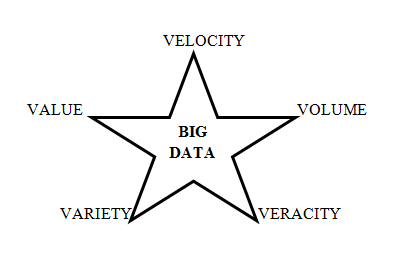
\includegraphics{bigdata.PNG}
\caption{Properties of Big data\label{overflow}}
\label{f1}
\end{figure}\\
As the development in  information technology  is in a rapid manner, there is  also a significant increasing  in volume of data. Big data is a buzzword used to describe a massive amount of both  structured and unstructured data that is so large that it's difficult to process using traditional database  and techniques[12]. In most enterprise scenario the data that is too  big or it moves too fast or it exceeds current dealing  capacity. Big data has the potential to guide the companies  improve operations and make faster, more intelligent  divisions. Collecting large amount data from sensor nodes  is the major concern in the field of information and  communication technology. Individual sensor nodes may  not provide accurate information. Therefore collecting  data from multiple sensor nodes is very essential. Now a days  gathering and analysis of Big data is an important  task Since as  the world of internet and technology is developing rapidly, the significance of big data is inevitable. The big data gathering is illustrated in Figure.\ref{f1} [1].
\\
\begin{figure}[ht!]
\centering
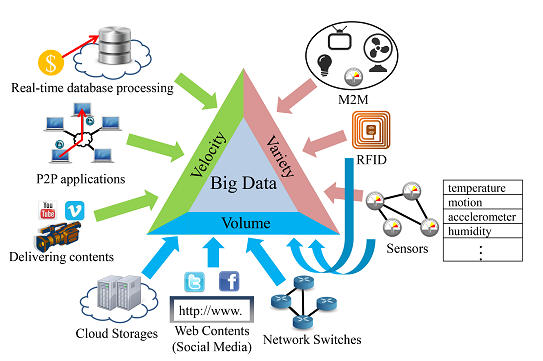
\includegraphics[scale=0.8]{bigdata2.PNG}
\caption{Big data Gathering\label{overflow}}
\label{f1}
\end{figure}\\
Wireless Sensor Networks is one of the main contributors of big data. Wireless sensor network is a collection of sensors which are communicating wireless. Sensor networks are highly distributed networks of small, lightweight wireless node, deployed in large numbers to monitor the environment or system. The wireless sensor network can be deployed in an environment to monitor the environment and alarm or notify the up normal behaviour or conditions of the environment. When sensors are distributed in an environment, it can monitor physical or environmental conditions, such as pressure, temperature, humidity, sound etc. Sensors have an advantage that it can be used in applications where human intervention could not be possible. Wireless sensor networks have many applications in military , medical, civilian, environmental monitoring, air pollution monitoring, forest fire detection, land side detection, water quality monitoring, air pollution monitoring, forest fire detection, landslide detection, water quality monitoring, nature disaster prevention, structural health monitoring etc[1]. A sensor is built with several components :radio transceiver with an internal antenna, an electronic circuit for interfacing with the sensors and an energy source such as battery [17].


                 Data dissemination and data gathering are two important operations in wireless sensor networks. Data gathering is the process of the collection of observed data from the individual sensor nodes to a sink. There are two problems in gathering the data sensed by sensors. First, the network is divided to sub-networks because of the limited wireless communication range. This limited communication range causes a challenge for data collection from all sensor nodes. For example, sensors deployed in a building may not be able to communicate with the sensors which are distributed in the neighbouring buildings. So that, limited communication range may pose a challenge for data collection from all sensor nodes. Second, the wireless transmission consumes the energy of sensors. Even though the volume of data generated by an individual sensor is not significant, each sensor requires a lot of energy to relay the data generated by surrounding sensors. Especially in dense WSNs, the life time of sensors will be very short because each sensor node relays a lot of data generated by tremendous number of surrounding sensors. So an energy efficient method is needed to gather huge volume of data from large number of sensors in wireless sensor networks.
               

 Mobile sink approach is an energy efficient way to gather data while deal with the divided sub network problem and energy consumption issue. In this approach sink node is assumed to be mobile such and as the sink node moves around the sensing area, the sensor nodes send data to the sink node when the sink node comes in their proximity. Thus, energy consumption can be decreased by reducing the amount of relays in the WSN. The sink node divides the sensor nodes into a number of clusters based on a certain condition. Then, the sink node roams around in these clusters. In  a network which consists of a mobile sink and many sensor nodes spread within a limited field, Every node (sink and sensor) has a limited communication range R and communication is always successful if it is within R. The mobile sink node patrols the cluster centroids that are calculated to minimize energy consumption for data transmission, and collects data from sensor nodes. Sensor nodes are equipped with a buffer memory and store sensed information until mobile sink approaches the cluster centroid. The information is transferred to the sink node by multi-hop fashion. Centroid of a cluster is the position in which the mass of a cluster is concentrated. In a sensor networks sensor node will gather data and store it in the buffer memory, the mobile sink will move towards the centroid of each cluster and gather that data and then send it to the base station for further processing
\section{Motivation}
We can clearly say that mobile sink is an energy efficient method to gather big data in wireless sensor networks. But the literature does not focus on the number of mobile sink which are required for a wireless sensor network with given number of sensor nodes. But we know the number of mobile sink have a high significance on the performance of energy consumption. If we are using less number of mobile sink for given number of sensor nodes, it will both time as well as energy consuming process. On the other side, if we use more number of mobile sinks than the required number, then surely there will be resource underutilization. Since sensor nodes are costly this approach is not a cost effective one. So it is important to find out the number of mobile sink which are required to gather data from a wireless sensor networks for a given number of sensor nodes.
\section{Thesis Organization}
This thesis is organized as follows. Chapter 2 gives the scope and objective of the proposed system. Chapter 3 describes the problem statement. Chapter 4 gives the literature review which describes various clustering algorithms and data gathering techniques in wireless sensor networks. Chapter 5 gives the system design  in which existing and proposed systems are analysed and the design of proposed system explained in detail. Chapter 6 shows results analysis of proposed system and performance evaluation is given. Chapter 7
gives the conclusion of the proposed system and future works.

\clearpage
\pagebreak
\chapter{SCOPE AND OBJECTIVE}
\label{chap:scope}
The world around us is changing every day in every aspects. Now a days each and everything is computerized. The areas of information and technology are two important factors that concerns with today's world. We are not using equipment or traditional devices that we had used say 10 years ago. Technology developed such a manner that it affect the social, economic life of humans. The influence of technology in society is like two sides of coin. There is some disadvantages regarding the social behaviour of people after the development of technology. But besides that the most important  and interesting fact is that technology made the lifestyle of today's world an easy one. This rapid development in technology has resulted in explosive growth in the  volume of data.


 As technology and internet are growing the amount of data produced is significantly high. These type of large data which cant handle using the traditional programming paradigms is termed as BIG DATA. Big data as the name depicts it is the data with high volume together with high velocity and variety. Now a days the role of big data is inevitable. So government, industries, academia are paying more attention towards big data. Since it can't be handled using normal methods the gathering, processing, analysing of big data need careful attention. Big data gathering thus make sense in this era.


	When it comes to the contributors of big data, there are many contributors like wireless sensor networks, web contents, social media, real time data processing etc. Among these wireless sensor networks play an important role. Even though data sensed by individual sensor is low, overall data generated by sensors in a large densely distributed  sensor network is very high. The application of  wireless sensor networks in our day to day life is also play an important role. For example, wireless sensor networks can be deployed in smart houses, industries, offices for sensing temperature,  humidity, pressure etc. These type of application produce wide variety of data in large volume. So the gathering of this data from wireless sensor network sounds important.
	
	
	In order to gather the data produced from wireless sensor network sinks are used. Since energy consumption is an important constraint in wireless sensor network, mobility factor is added to  the sink for collecting data from the sensor nodes. So the mobile sink will move towards sensor nodes and collect data from it. Mobile sink approach is an important step towards the data gathering in wireless sensor network. Energy consumption can be reduced by using this approach. Detailed study of mobile sink approach can leads to some important findings that can make the data gathering process easy in future.

\pagebreak
\chapter{PROBLEM STATEMENT}
\label{chap:problem}
 The main problem faced by wireless sensor network is the energy consumption. Due to the wireless transmission and limited communication range a lot of energy is consumed in wireless sensor networks. Data gathering using wireless sensor network also face this constraint of energy. The number of mobile sink is an important factor since it can greatly influence the consumption of energy. Mobile sink approach is an effective way to gather data from wireless sensor network in an energy efficient manner. Sink is used to collect data from the sensor nodes and further forward it to the base station for processing. In mobile sink approach, the sink will move towards the sensor nodes and collect the sensed data. The amount of relays in wireless sensor networks can be reduced by using this approach. In effect the energy consumption can be reduced.
 
 
For a wireless sensor network with given number of sensor nodes  we don't know the required number of mobile sink for gathering data in an energy efficient manner. If we know the number of mobile sinks which is needed to gather data from a given networks resource underutilization  can be avoided. In addition to that gathering can be performed in a cost effective manner
 
 
 So here the problem is that how many number of mobile sinks can gather data energy efficiently from a wireless sensor network for a given number of sensor nodes. The earlier work concentrated on static wireless sensor networks. Now a days most of the wireless sensor networks are dynamic. So it is equally important to experiment this problem in a dynamic environment. So put it in a nutshell, the problem is to find out the number of mobile sinks that can gather data in an energy efficient manner from a dynamic wireless sensor networks when the number of sensor nodes are fixed

\pagebreak
\chapter{LITERATURE REVIEW}
\label{chap:lit}
Big Data is a fuzzy which represents amount of data that exceeds
the processing capacities of conventional systems[15]. Big Data is still a maturing and 
evolving discipline. Big data databases and  files have scaled beyond the capacities and  capabilities of commercial database  management systems[16]. Some literature about Big data reviewed here


In [13] saigiroglu et al. found that Massive data which have large and complex structure is termed as bigdata. Big data is difficult to store, analyse and visualise. Online transactions, emails, videos, audios, images, click streams are contributing to big data. Since these data are of large volume, it is difficult to capture, form, store, manage, share, analyse and visualise by using traditional tools. Big data has mainly three properties velocity, volume and variety. There are mainly three varieties of big data sources structured, semi structured and unstructured. Volume of data is significantly large than terabytes and petabytes. Big data itself and processing of big data is with high velocity .Big data samples available are astronomy, genomics, life sciences etc. Generally the potential of big data  distributed in five topics Health care, Public sector, Retail, Manufacturing , Personal location data. One important method for big data processing is Map-Reduce model. Map Reduce is a programming framework  for distributed computing which was created by Google. Then a  java based framework Hadoop developed by getting inspiration from Google's Big Table. In short this paper presented the overview, scope, samples, methods of Big data.


The term Big data has very important role in health informatics and biomedical areas[14]. This paper presents the role, important and development of Big data in health care and biomedical areas. The Area of health is concerned with too big, too fast, and too complex datasets which is difficult  for healthcare providers to process and interpret with existing tools. So here comes the importance of Big data in health. Big data have six properties value, volume, velocity, variety, veracity  , variability which also applicable to health data. Big data helps to boost the applicability of clinical research studies into real-world scenarios, where heterogeneity of population is a constraint. It equally provides the opportunity to enable effective and precision medicine by performing patient stratification. This is indeed a key task toward personalized healthcare. Future clinical research relies on the advancement in big data processing for healthcare informatics, bio-informatics. The rapid and seamless health data acquisition contributes towards the importance of big data in medicine.


In [15] Rios and Diguez addressed  the integration of big data tools for gathering, storing and analysing data generated from the wireless sensor networks. Data  generated from large scale wireless sensor networks are exponentially high. The data generated from wireless sensor networks can be processed using conventional technologies. But as the volume of data increases these methods are not cost effective. Most importantly, they cannot cope with the processing needs that can be required for real-time processes where WSN have been deployed in natural disaster, fire detection and traffic control. New tools are emerging for  the gathering and processing of Big data. These tools can capture, process, store, transfer, search, publish, analyse and visualise large data generated by wireless sensor networks. When we implement systems where these two technologies co-exist, there are certain challenges due to the complexity of concepts and variety of tools. In order to  understand and address  these challenges, this paper   build a platform that integrates a WSN and a distributed processing and storage system. This system was completely developed with open source tools. A prototype is implemented here for reading, processing and analysing sensors in real time. Open source technologies like storm and Hadoop used for developing the prototype.
\newpage
Wireless sensor network  is network of sensor node which is distributed in wireless manner. Wireless sensor network consist of sensor nodes and base station. These types of networks are  deployed for monitoring an environment or system. Limited energy and bandwidth are two constraints of wireless sensor networks. An energy-efficient, scalable approach to reducing the energy consumption over the whole network is the clustering process. It also increases network lifetime. When clustering is applied in wireless sensor network, nodes are divided into multiple clusters, and a head node will be assigned for each cluster as a leader, which collects all the data from the sensors belonging to its cluster and relays these data to the sink node directly or by multiple hops[6]. Different methods and algorithms are proposed for clustering in wireless sensor networks. Some works are reviewed and summarised here.


In [2] Dynamic Clustering Routing Considering Load(DCRCL)Is proposed for clustering. It addresses the problem associated with leach. In leach, there is a chance to select a low energy node as cluster head. Another problem is that communication between cluster head and base station is in a single hop manner which will consume more energy and thus reduce the network life cycle. Even though large number of algorithms like PEGASIS, HEED are developed to overcome this problem, data delay is high and it is not suitable for large sized networks. Even though these algorithms can improve the total lifetime of the network, the load problem is not addressed.
	In DCRCL the load problem is addressed. The algorithm consist of mainly three phases. Cluster head selection, Cluster set up and inter cluster routing. Residual energy and node load is considered for cluster head selection. In cluster set up phase in order  to avoid  the unbalanced distribution of cluster heads in LEACH, cluster head competitive mechanism is used. That is after being candidate cluster head, the node competes with other candidates in its communication range and the one with highest residual energy will be selected as cluster head. In the third phase, inter cluster routing  it addresses the problem with LEACH. In Leach data transmitted directly from cluster head to base station which reduce the life cycle of cluster head as well as network. In DCRCL, energy balanced clustering communication model is established for efficient use of network model


In [3]  Prasanth Krishnan et al. compared the performance of different static as well as dynamic clustering protocols. The performances are evaluated using various node distribution schemes like Random node distribution, Poisson distribution and Uniform distribution. Routing is the process of determining the path between source and destination. There are many types of routing protocols on the basis of different parameters. When it comes to wireless sensor networks, the routing protocols are mainly classified into flat, hierarchical based routing and location based routing. In hierarchical, nodes in the network have different roles. It can be further classified in to two, static and dynamic. In dynamic, cluster are dynamic in nature but in Static, once the clusters are created remain same throughout  network lifetime. Prasanth et al. compare the  performance of LEACH,  Enhanced  Energy-Efficient Protocol with Static Clustering (E3PSC) and Energy-Efficient Protocol with Static Clustering(EEPSC). The Low Energy Adaptive Clustering Hierarchy (LEACH)  is Dynamic Hierarchical  Routing for sensor  network. In LEACH the selection of cluster heads will be in a random manner. Cluster head will compress and aggregate data that are coming from cluster nodes and send this data to the base station. LEACH uses a TDMA/code-division multiple access (CDMA) MAC to reduce inter-cluster and intra-cluster collisions. When constant monitoring to the network is needed LEACH is the most appropriate solution. In LEACH there are two phases, the setup phase and the steady phase. In the set up phase, the cluster  organization  and cluster head selection takes place. In the steady state phase, the actual data is  transferred  to the BS. For minimizing the overhead the setup phase is less durable as compared to steady phase. The problem with LEACH is that it is not applicable to large networks. It also assumes that nodes always have data  to send, and nodes located close to each other have  correlated  data. Performance analysis depicts that nodes over poisson  random distribution are alive for maximum network lifetime. Network lifetime of  Nodes deployed on uniform random number distribution is less than network lifetime of nodes deployed on poisson distribution. The second protocol, Enhanced  Energy-Efficient Protocol with Static Clustering  (E3PSC)  is an improvement of an existing routing scheme, Energy-Efficient Protocol with  Static Clustering (EEPSC). In this protocol, Spatial distribution of sensors nodes in network and their  residual  energy are considered for selecting cluster head. This will  reduce the  communication overhead within cluster. Performance analysis shows that  E3PSC  will provide good result in uniform random distribution. In  Energy-Efficient Protocol with Static Clustering, it eliminates the overhead of dynamic clustering  by dividing the network into static clusters. It distribute the energy load among high power sensor nodes by using temporary-cluster-heads. In effect it  extends network lifetime. There are three phases in EEPSC, set-up phase, responsible node selection phase and steady-state phase. Static clustering Scheme and  idea of temporary cluster heads  are the advantages of this protocol.


In [4] Benkirane et al. proposed WDDC[Weighted Dynamic Distributed Clustering), which is based on the ratio of residual  energy and average energy of the network. This approach  takes into consideration distances between nodes  and the base station to determine near nodes and distant nodes in order to give more chance to  the nearest nodes to be cluster heads by modifying  the election probability value for every type  of nodes. WDDC is dynamic approach and it is autonomous as well as more energy efficient. It increases the lifetime of networks. In WDDC, nodes with more energy than the other nodes and the nodes with less distance  from the BS have more chance to be selected as a cluster-head for current round. So this approach introduced a concept of weighted probabilities for every type of nodes according to their residual energy and the average energy of the network in current round. The distance between nodes and the base  station are also taken into consideration  for favouring the  nodes with more  energy and closest to the BS to become cluster heads. The method of communication between cluster head s and cluster nodes are similar to LEACH. That is After the cluster head formation, it will inform all other nodes about its selection as cluster head. After that other nodes choose the most appropriate cluster heads and organize themselves into local clusters. Then cluster head gets data from the cluster nodes according to TDMA Schedule. When it comes to the communication between cluster head and base station, after  receiving all the data from the cluster nodes, the cluster head node executes signal 
processing functions to compress the data into a single signal. Then  each cluster head  send the combined data to the base station. The consumed energy of cluster head is composed of three parts: data receiving, data  aggregation and data transmission. The main advantage of WDDC is that it have significantly high stable time which increases the  efficiency of networks. In addition WDDC consumes less energy when compared to other protocols. So network lifetime can be increased.


Deepali virmni et al. proposed  a  dynamic cluster formation method where clusters are refreshed periodically based on residual energy, distance and cost in [5]. Here distance is   considered in order to minimize energy consumption and increase  lifetime of the network. The main focus is to minimizing energy conservation, maximizing network lifetime, and real time communication. A dynamic clustering protocol (DSP) is proposed  which forms the cluster based on the residual energy of each node. The concept of assigning different energy levels to different nodes is introduced  for  balancing the responsibility among the cluster nodes. The node with the highest energy level looks for nodes within its transmission range forms a cluster and  appoints itself as the cluster head  of the cluster formed. Then data transmitted from all the cluster nodes to the cluster head. That is cluster head act as a data aggregating node in for its respective cluster. After sending data to the cluster head nodes will go to sleep state until they have something more to transmit. Only Cluster head communicate with other cluster head thus reduces the energy consumption. So in effect the  lifetime of node  increased. After data aggregation cluster head forward the data to base station. This step reduces the energy of the cluster head. So calculation of remaining energy and election of cluster heads are conducted in periodic intervals. Here clustering can be performed even though the position and energy of nodes are changing. This dynamic clustering will results in the effective energy utilization of all the nodes in the network. In short here proposed protocol  is better in terms of energy conservation and enhancement of network life time as sleep and wait technology enhances the 
lifetime of nodes.


In [6] a simple-but-effective routing tree Algorithm is proposed  to maintain a dynamic energy efficient tree structure over all cluster heads, in order to further reduce the energy consumption for those heads to relay data to the sink. Two challenges in clustering based communications are balancing the overload over all network nodes as well as the energy budgets inside clusters, and reducing the significant energy resulted from heads that relay data
to sink over a distance-long link. To address these two problems, this study proposes a clustering based hierarchical protocol. With a k-medoids clustering scheme, the proposed protocol can lead to a set of evenly-distributed clusters, effectively balancing the overload of the network. It further increases the energy efficiency inside the cluster. Simple-but-effective head update policy also designed in this paper. Also a  method of constructing and maintaining a dynamic routing tree over all cluster heads is also included. Traditional clustering algorithm for wireless sensor network selects cluster heads  firstly and then form the cluster by allowing non-head nodes connect to some head. The proposed clustering uses the inverse procedure. K-medoid clustering  scheme is used to divide the nodes into different clusters, then one node from each cluster will be selected as cluster head. This method provide traffic balance, increase network life time and reduced execution cost. Here k-medoid algorithm is used to divide the nodes into k distinct clusters. The basic idea is the continuous iterations until a set of heads is figured out such that these heads distribute evenly within the network area and all clusters are about the same in the number of member nodes. 
A Location-Aware Broadcast scheme at MAC level (LAB-MAC) is proposed to save both the energy and the bandwidth in order to select heads efficiently. A simple and computation less method I used here for updating cluster heads. Many traditional clustering algorithms, like LEACH,
are two-layer hierarchical networking, that is, the cluster heads transmit data directly to the sink, which significantly consumes head's energy due to the distance-long communications. For solving this  issue, this paper constructs a dynamic routing tree for all heads to improve the energy efficiency by reducing the transmit power of heads. In addition  intra-cluster head update policy used to  change  heads dynamically and thus balance the energy consumption of cluster nodes.


In [7] Anker et al. proposed a useful fully-distributed inference algorithm  for clustering, based on belief propagation. The attention to the performance of the multi-hop network was quite limited while most works  have focused on an energy-efficient clustering scheme. An energy-efficiency algorithm may select a few cluster heads for energy-saving, but if these CHs do not have good connectivity or if they are not stable, the retransmission and the dropped packets may significantly degrade the network
performance and the total energy wasted will be higher. Therefore, taking reliable communication into account is essential for any clustering algorithm which aims to reduce the energy consumption in a network. Moreover, the network lifetime should be measured not only by the time that
the first or the last node dies, but also by the period of time that the network is available for providing services and operating appropriately. Since the network is usually dense and many nodes are redundant, the death of a few nodes does not affect the network. Thus, network lifetime is tightly coupled with the network performance. This paper solves the clustering problem
in multi-hop networks with a special focus on network performance, using the belief propagation (BP) algorithm. It is an iterative algorithm for computing marginal probabilities on trees, by local message passing. The main advantage of this method over existing algorithms for clustering is
that BP considers not only local properties of a node, such as residual energy or degree, but also takes into account joint characteristics of a group of nodes, such as link quality and topology information. Utilization all available data, while maintaining small constant message and time overhead, leads to considerable increase in network performance and balanced power consumption among the nodes. This paper proposes new algorithm for efficient clustering that considers  the power balancing among the nodes as well as  the total transmission power aggregated in the multi-hop routing. This paper also  presents a scalable and practical implementation of BP in WSN for inference goals. Proposed algorithm has advantages like  improving the data transmission time and rate.


In [8] Khara and Sasikumar proposed a centralized and  distributed k-means clustering algorithm. k-means algorithm is based mainly on the Euclidean  distances and cluster head selection depends on residual energies of nodes. So here the central node collects the  information about the node id, position and residual energy of  all nodes and stores this information in a list in the central 
node. After getting this information from all nodes it starts performing the clustering algorithm (k-mean). It proposed both centralised and distributed k-means clustering algorithm.
Centralized way of clustering is a method of clustering in which  a centralized authority makes decisions and partitions of  the nodes into clusters without the involvement of other nodes. Here the centralized authority  gets the necessary information for clustering from the 
individual nodes. Based on this information it will cluster  and sends the clustering results back to the individual nodes. If  every node in the network  participates in making clustering decisions, it is a distributed way of clustering. Here every node  gets the necessary information for clustering from all other  nodes. Based on this information all nodes will cluster and also decides the cluster head.
Since the k-mean algorithm  is based on Euclidean  distances and energies  the information about the positions and energies of all nodes is  obtained by every node by exchanging messages among  themselves. After getting the information about all nodes every  node runs the algorithm (k-mean). From the simulations  it is clear that the network is more stable for distributed clustering when compared to centralized clustering.


A.B.M.Alim et al.[9]  presented   Stable Sensor Network (SSN) to achieve balanced energy consumption 
rate using dynamic clustering to guarantee stability in WSN. Lifetime of wireless sensor network  can be defined  as stability period of WSN when it considers the time required for the first sensor node to die. There is an impact of efficient usage of available energy in a sensor  node on stability period of WSN. This period is mainly controlled by balanced energy consumption rate throughout the network. Therefore, it is necessary  to ensure balanced use of the available energy throughout the network along  with the efficient use of the available energy in a sensor node to assure stability in WSN. This paper proposed a novel technique Stable Sensor Network (SSN), which ensures balanced use of the available energy  throughout the network. It also achieves the efficient use  of the available energy in a sensor node by exploiting  clustering technique and   proved that SSN has a significant  improvement in network stability over LEACH. SSN is a self-organising and adaptive clustering protocol. Three heuristics for SSN is used in this paper with proper justifications
The summarization of related work is given in Table.\ref{table1}
\\
\begin{table*}[h]
\scriptsize\addtolength{\tabcolsep}{-4pt}
\centering
\caption{\label{table1} Comparative study of Related works on Clustering}
{
\hfill{}
\begin{tabular}{|p{0.3\linewidth}|p{0.25\linewidth}|p{0.20\linewidth}|p{0.20\linewidth}|}
%\begin{tabular}{|l|l|l|} 
  \hline
 \textbf{Name of Paper } & \textbf{Description} &\textbf{Merits} & \textbf{Demerits} \\ 
\hline  
\vspace{5mm}
Research on Dynamic Clustering Routing Considering 
Node Load for Wireless Sensor Networks[Yi Sun, Can Cui, Shanshan Ke, Jun Lu, 2013]
&\vspace{5mm} Proposed an clustering algorithm that considers network load and residual energy &
\vspace{0.7mm}
* Efficient
 
* Addresses the problems of LEACH 
  
* Increases the life cycle of network
 
 
* Increases the data volume of network

&\vspace{0.7mm}
* Nodes are static 
 \\
\hline
\vspace{5mm}
Comparison and Performance Analysis of Dynamic 
and Static Clustering Based Routing Scheme in 
Wireless Sensor Network[Prasanth Krishnan, 2013]
&\vspace{5mm} Compared the performance of different static as well as dynamic clustering protocols. &
\vspace{0.7mm}
* Using various node distribution schemes used for evaluation
&\\
\hline
\vspace{5mm}
Weighted Dynamic Distributed Clustering 
Protocol For Heterogeneous Wireless 
Sensor Network[Said Benkirane, 2012]
&\vspace{5mm} Proposed an autonomous, efficient and dynamic algorithm for clustering &\vspace{0.7mm}
*High Stable time

* High efficiency

* Less energy consumption

* Increased network lifetime

* Heterogeneous WSN
 
&\vspace{0.7mm}
* Sink is static 

* Sensor nodes are static
\\
\hline
\vspace{5mm}
Dynamic Clustering Protocol for Data Forwarding in 
Wireless Sensor Networks[deepali virmani ]	
&\vspace{5mm} Proposed a dynamic cluster formation method&\vspace{0.7mm}
* Increased network life time 

* Enhanced energy conservation

&\vspace{0.7mm}
* Delay 

* Didn't support real time parameters
\\
\hline
\vspace{5mm}
Dynamic Cluster-based Routing for Wireless
Sensor Networks[Lin Zhao, 2014]		

&\vspace{5mm}Proposed simple-but-effective routing tree
algorithm to maintain a dynamic energy-efficient tree structure over all cluster heads&\vspace{0.7mm}
* Even distribution of cluster heads
 
* Balance energy consumption 

* Increased network life time
&
* Delay 

* Static clustering 

* Didn't consider unreliable links
\\
\hline
\vspace{5mm}
Efficient Clustering for Improving Network
Performance in Wireless Sensor Networks[Tal Anker]	 
&\vspace{5mm}Proposed a useful fully-distributed
inference algorithm for clustering, based on belief propagation.&
\vspace{0.7mm}
* Increased throughput
 
* Minimize overall transmission cost

* Longer lifetime	

&\vspace{0.7mm}
* Delay 

* Communication Load is comparatively high
\\
\hline
\vspace{5mm}
K-Means Clustering In Wireless Sensor Networks[P.sasi kumar, 2012]
	 &\vspace{5mm}Proposed centralized and 
distributed k-means clustering algorithm&
\vspace{0.7mm}
* Distributed clustering is  more efficient	
 
&\vspace{0.7mm}
* Delay 

* High energy consumption
\\
\hline
\end{tabular}}
\hfill{}
\end{table*}

Data gathering is an important operation of wireless sensor network. It is the process of collecting data from various sensor nodes to a sink node further to the base station in a network. Various methods used for data gathering in wireless sensor networks are summarized here


Rashmi et al.[10] proposed  data-gathering technologies for large-scale  wireless sensor networks by introducing mobility into the network. An M-collector (mobile data collector) starts  the data-gathering tour periodically from the static data sink, polls each sensor while  traversing its 
transmission range, then directly collects data from the sensor in single-hop communications, and finally  transports the data to the static sink. It actually focused  on the problem of minimizing the length of each data -gathering tour and refer to this as the single-hop data-gathering problem (SHDGP).
An Algorithm is proposed for  data-gathering  where multiple M-collectors traverse through several shorter sub tours concurrently to satisfy the  distance/time constraints. The aim of the proposed approach  is to achieve energy efficient Data Collection in densely distributed Wireless sensor  networks using Mobile Collector. For clustering the k-medoid algorithm is used. New data-gathering mechanisms for large-scale sensor networks when single or multiple M-collectors are used proposed in this work. In this data-gathering scheme with multiple M-collectors, only one M-collector needs to visit the transmission  range of the data sink. While the entire network can be divided into sub networks. In each sub network, an M-collector is responsible for gathering data  from local sensors in the sub area. Once in a while, the M -collector forwards the sensing data to one of the other nearby M-collectors, when two M-collectors move close enough. Finally, data can be forwarded to the M-collector that will visit the data sink via relays of other M-collectors. All 
data are forwarded to M-collector 1 from other collectors, and then, M-collector 1 carries and uploads data to the data sink. Proposed method can prolong the network life time significantly compared with the scheme that has only a static data collector and scheme in which the mobile data collector can only move along straight lines.


Liu et al. studied  the transport capacity of a data-gathering wireless sensor network under different communication organizations in [11]. The reason for considering many-to-one type of
communication among other possibilities is because many-to-one and many-to-few  are communication modes that commonly take place in a data-gathering wireless sensor network. Communications within each cluster are of the many-to-one type, i.e, data flows from each sensor
to the cluster head where they can be processed, compressed, aggregated and relayed. Within the context of many-to-one communication, possible organizations of the network include the flat and hierarchical organizations. In a flat organization all nodes/sensors act as peers in transmitting and relaying data for one another. In a hierarchical network, layers of clusters are formed.
Nodes send their data to the cluster heads who then relay the data to either a higher layer cluster head or the sink. This paper examine and compare both organizations in terms of transport capacity and energy consumption. Many-to-one throughput capacity is defined 
as the per source data throughput, when all or many of the sources are transmitting to a single fixed
receiver or sink. Since many-to-one communication causes the sink to become a point of traffic concentration, the throughput achievable per source node in this case is reduced. This paper concentrated in  the case where every source gets an equal  amount of original data across to the sink. Equal share of throughput from every sensor is desired for applications like imaging where each
sensor represents a certain region of the whole field and data from each part are equally important.
When distributed data compression is used this is again approximately the case. However,
when conditional coding is used this may no longer be true since the amount of processed data
can vary from source to source. This paper derived an upper bound as well as constructive lower bounds for both the flat and the hierarchical network architecture.


In [12] Vijayalaxmi  proposed a  method for  establishing sink routing and clustering method based on k-medoid  algorithm. The big data has become a popular topic because of enormous growth in the field of information technology. The distributed sensor network is the production of big data. A single sensor in a network may not give a significant  data, but the data  sensed by millions of sensors produce a big data. Big data gathering in densely distributed sensor  network with energy efficiently is a challenging task. In order to gather these data, the WSN is constructed in  such a way the sensors relay their data to the "sink". This paper  focused on efficient big data gathering from heterogeneous 
wireless sensor networks. In traditional clustering algorithm at the first step cluster heads are selected and then clusters are formed. But in proposed algorithm at the first phase the nodes are divide into  distinct  clusters with k-medoid clustering scheme and  then one node inside each cluster will be selected as a cluster head. In short paper  introduced a robust algorithm for big data gathering using k-medoids algorithm. The k-medoid clustering  is reliable clustering algorithm in reducing power  consumption mainly for network with large number of  sensor nodes. It  is also a effective algorithm in  selecting centroid.
The summarization of related work is given in Table.\ref{table2}
\begin{table*}[h]
\centering
\caption{\label{table2} Comparative study of Related Works on Data Gathering}
{
\scriptsize\addtolength{\tabcolsep}{-5pt}
\hfill{}
\begin{tabular}{|p{0.3\linewidth}|p{0.3\linewidth}|p{0.2\linewidth}|p{0.17\linewidth}|}
%\begin{tabular}{|l|l|l|} 
  \hline
 \textbf{Name of Paper } & \textbf{Description} &\textbf{Merits} & \textbf{Demerits} \\ 
\hline  
\vspace{5mm}
Energy Efficient clustering techniques for Mobile Data Gathering in Distributed WSN[Rashmi KR, 2015]	
&\vspace{5mm}Proposes data-gathering technologies for large-scale  wireless sensor networks by introducing mobility into the network. &\vspace{0.7mm}
* Efficient

* Increased network life time

* Mobile collector 
&\vspace{0.7mm}
* Time consuming


*Energy of mobilesink will reduced 
 \\
\hline
\vspace{5mm}
Data-gathering wireless sensor networks: organization
and capacity[Enrique J. Duarte-Melo, 2003]		
&\vspace{5mm}Studied  the transport capacity of a data-gathering wireless sensor network under different communication organizations &\vspace{0.7mm}
* Derived an upper bound  and lower bound 

* Used flat and hierarchical  architecture 
&\\
\hline
\vspace{5mm}
An Efficient way to Gather Big Data in WSN 
using Mobile Sink Routing[vijaya laxmi, 2015]	
&\vspace{5mm}
* Established  sink routing and clustering method based on k-medoid 
algorithm. &\vspace{0.7mm}
* Heterogeneous nodes 

* K-medoid algorithm is used for clustering	
&\vspace{0.7mm}
* Time consuming
\\

\hline
\end{tabular}}
\hfill{}
\end{table*}
\pagebreak

\chapter{SYSTEM DESIGN}
\label{chap:sysstud}
Data gathering using wireless sensor network face the two challenges. First due to the limited communication range, the network is divided to sub-networks. The second challenge is wireless transmission consumes energy of clusters. So for address these challenge in the wireless sensor network an energy efficient method is needed to gather data from wireless sensor networks.


The system is mainly designed to overcome the energy consumption issues during data gathering in Wireless sensor network. Mobile sink approach is used to solve this problem. The sink or the data collector in this approach is  assumed to be mobile. As the sink node move around sensing area, the sensor node send the sensed data to sink node. The sensor nodes in the network are divided into clusters based on modified clustering algorithm. Then sink node move towards each cluster to collect data. The whole mass of a cluster is concentrated in centroid. The sensors in wireless sensor network is organized as clusters Mobile sink gather data from the centroid of clusters in WSN.


	 Earlier work proved the fact that by using modified EM(Expectation Maximization) algorithm with mobile sink based clustering and data gathering will solve these issues and introduce a new relationship that will further reduce the energy consumption and cost effective with better performance. The expectation maximization method for clustering aims to minimize the sum of square of wireless communication distance. The main aim of this clustering scheme is to maximization of the expecting gain. For that it will use the distance property so it will reduce energy consumption by reducing the communication distance. That means nodes which are closest will form a cluster. Thus there are so many clusters are created in which nodes within cluster are of shortest distance than from the nodes between the cluster. In that case the sensor nodes were static, so distance calculation and application of EM algorithm was possible to do. But when it comes to our case, the sensor nodes are dynamic in nature. The previous approach is not applicable in the dynamic environment. The distance is not a static value in this case. So the EM algorithm can't be used here for clustering and centroid calculation.


	Considered network topology is a heterogeneous one as shown in Figure.\ref{f3}. Topology consists of mobile sink, base station and sensor nodes. Here the Sensor nodes are not homogeneous. They are heterogeneous in nature. That is some of them have high battery power while some not. There are two types of sink in the proposed topology, static sink and mobile sink. Static sink is nothing but the cluster head of each cluster. The basic idea is that Static sink will gather data from all of its cluster nodes and store it in the buffer memory,then the mobile sink will move towards the cluster head that is static sink of each cluster and gather /collect data from it. Later on the mobile sink will send this data to the base station.\\
\begin{figure}[ht!]
\centering
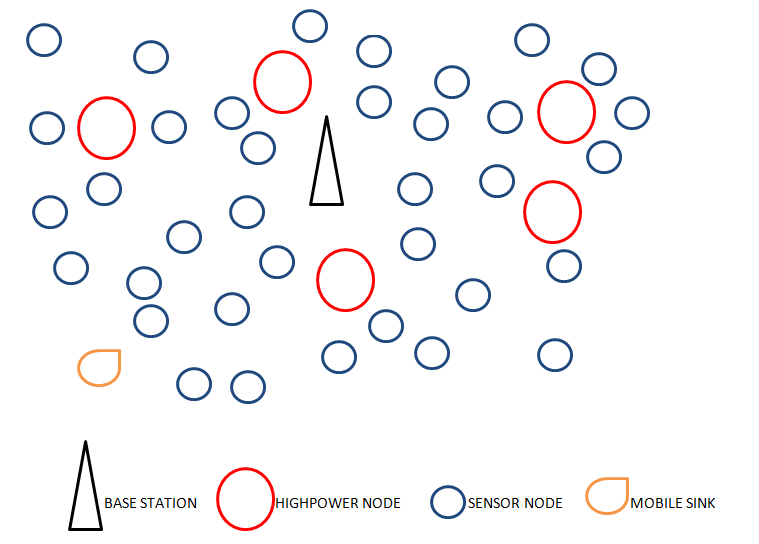
\includegraphics[scale=.75]{networktopology.PNG}
\caption{Network Topology\label{overflow}}
\label{f3}
\end{figure}\\
  For find out the number of mobile sink which is used to gather data from  a WSN for a given number of sensor nodes, here uses the two sink approach. The clustering and cluster head selection is somewhat a difficult task since sensor nodes are highly dynamic in nature. The high power nodes are selected as cluster heads and works as a static node by gathering data from the sensor nodes. After the deployment of network, the low power nodes will broadcast their presence to all other nodes which are inside their proximity.


When a high power node receives this broadcast, it will send a reply to the node which broadcasting the request. The node compare all replies from the high power nodes and choose the highest power node as its cluster head. If it get reply from one node only, that high power node is selected as cluster head. Then the node notify the cluster head about the selection. When cluster head node receives this notification about the selection, it will form a cluster with nodes from which it gets the cluster head notification. Cluster head of each cluster acts as static node. It gather data from all the cluster nodes. The cluster head will count the number of packets it gather and when it reaches a limit it will inform the mobile sink to collect data from it. When mobile sink receives this notification it will move towards the  cluster head and gather the data from it and then send it to base station. When a node leaves a cluster while moving it will send a notification to the cluster head. When all the cluster nodes has left from a cluster, cluster head will goes to a sleep state.
The  algorithm \ref{alg2} explains the  proposed algorithm for the clustering and cluster head /static sink selection .\\
\begin{algorithm}[t]
  \caption{Modified clustering algorithm with mobile sink based data gathering}
  \label{alg2}
  \begin{algorithmic}[1]
  \setstretch{1.35}
  \State{Start}
  \State{Deploy nodes in a heterogeneous manner }
\State{Each node broadcast  its  presence to all other nodes  within its sensing area}
\State{When a high power node receives this broadcast, it will send a reply to the  node}
\State{The node compare all replies from the high power nodes and choose the highest power node as its cluster head.}
 \State{Node  notify/inform the cluster head about the selection}
 \State{When cluster head node receives this notification, it will form a cluster with nodes from which it gets the cluster head notification}
\State{Cluster head of each cluster acts as static Sink. It gather data from all the cluster nodes.}
\State {The cluster head will count the number of packets it gather and when it reaches a limit it will inform the mobile sink}
\State {When mobile sink receives this notification it will move towards the  cluster head and gather the data from it}
\State {Mobile sink sends data to base station}
\State {When a node leaves a cluster while moving it will send a notification to the cluster head and repeat 3-11}
\State {When all the cluster nodes has left from a cluster, cluster head will goes to a sleep state.}
\State {The mobile sink gather information until no more cluster head is to send data}
\State {Stop}
\end{algorithmic}
\end{algorithm}
\newpage
\section{System Implementation}
The considered network consist of heterogeneous sensor nodes, mobile sink and base station. High power nodes will form cluster as explained in  \ref{alg2} and act as static sink. The sensor nodes gather data from its surroundings. The static sink is nothing but the cluster head of each cluster. It will gather data from sensor nodes and store it in the buffer memory. When the buffer memory is full, it will inform mobile sink. MS will visit the  static sink and gather data from its buffer  and send this data to the base station. The architectural framework for the implementation is shown in  Figure.\ref{f4}\\
\begin{figure}[ht!]
\centering
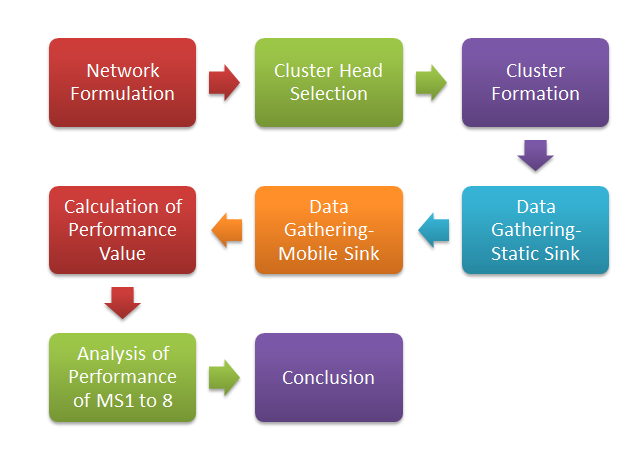
\includegraphics[scale=.8]{architecure.PNG}
\caption{Network Architecture\label{overflow}}
\label{f4}
\end{figure}\\
Network formation phase is used to deploy the sensor node in the field where monitoring is to be performed. The network topology consist of sensor node, mobile sink and base station. Nodes are heterogeneous in nature. Some nodes have high battery power while others are normal nodes. Mobile sink  have the ability to move towards each cluster head and collect data from it. One base station is deployed in each topology. After gathering data mobile sink will send data to the base station for further processing.


 In cluster head selection phase each low power node broadcast its presence to neighbours. The highest power node within the proximity receives this broadcast and send reply to the low power (normal) nodes. The normal node compare all the reply received from high power nodes and elect the highest power nodes as the cluster head. Then it will notify the highest power node about the selection.
 
 
  The cluster formation phase is used for the formation of cluster. The cluster is formed by the cluster head. That is after getting cluster head selection notification from a low power node, cluster head form a cluster  with all nodes from which it gets the cluster head notification. The nodes in the cluster senses the environment it deployed on and collect this data. Then nodes within the cluster communicate with static sink when the it senses data. That is sensed data from the cluster nodes are collected by the respective cluster head or static sink of each cluster. The static node or Cluster head has a fixed buffer size. When the buffer of static node is full it will notify mobile sink. Mobile sink then visit the static node and gather data from it. The collected data further send to base station in each topology.


Performance evaluation is done by creating the seven topology each with one to seven mobile sink for data gathering with same number of sensor node. That is create topologies with fixed number of sensor nodes and vary the number of mobile sink in each topology. Modified clustering MS based data gathering is implemented in each topology. Then data gathering  performed and collected data by mobile sink send to base station.


 Analysis phase is used for the analysis of each topology against the following performance parameters: packet delivery ratio (PDR), residual energy, data transfer time, packet sent-received-dropped count, hop count and the number of MS used.


\pagebreak
\chapter{RESULTS AND PERFORMANCE ANALYSIS}
\label{chap:fut}
The performance evaluation is done in a simulated environment using NS2. The seven different  topology ranging from one to seven mobile sink is created.  Modified clustering and mobile sink based data gathering is implemented in each topology. Performance parameters are measured by using the awk script. Here the parameters considered are average packet delivery ratio, residual energy, data transfer time, packet sent-received-dropped count, hop count and the number of MS used.

\section{Tools Used}
\subsection{NS2}
NS (Network Simulator) is a discrete event simulator targeted at networking research. 
NS provides substantial support for simulation of TCP, routing, and multicast protocols over 
wired and wireless (local and satellite) networks. Network simulators are used to simulate 
behaviour  of network on a simulator. Simulation is a process in which an entire system 
is made functional in a hypothetical  manner with the help of simulation tool. NS2 is 
also one such simulation tool but its not just another simulator. It is used across the 
globe and is available free of cost. It is often used by researches to help evaluate the 
performance of new protocols  or validate analytical models. NS2 allows you to setup a 
computer network, consisting of nodes/routers and links. You can then send data (packets) 
over the network using a variety of different protocols at different layers.


NS uses two languages because  any network simulator, in general, has two different 
kinds of things it needs to do. On the one hand, detailed simulations of protocols require a 
systems programming language which can efficiently manipulate bytes, packet headers, and 
implement algorithms  that run over large data sets. For these tasks run-time speed is 
important and turn-around time (run simulation, find bug, fix bug, recompile, re-run) is less 
important. On the other hand, a large part of network research involves slightly varying 
parameters or configurations, or quickly exploring a number of scenarios. In these cases, 
iteration time (change the model and re-run) is more important. Since configuration runs once 
(at the beginning of the simulation), run-time of this part of the task is less  important. NS 
meets both of these needs with two languages, C++ and OTCL. C++ is fast to run but slower 
to change, making it suitable for detailed protocol implementation. OTCL runs much slower 
but can be changed very quickly (and interactively), making it  ideal for simulation 
configuration. NS (via TCL) provides glue to make objects and variables appear on both 
languages. 


Depending on the user's purpose for an OTCL simulation script, simulation results are stored 
as trace files, which can be loaded for analysis by an external application: 
\\
1. A NAM trace file (file.nam) for use with the Network Animator Tool
\\
2. A Trace file (file.tr) for use with XGraph or Trace Graph. 
\begin{figure}[ht!]
\centering
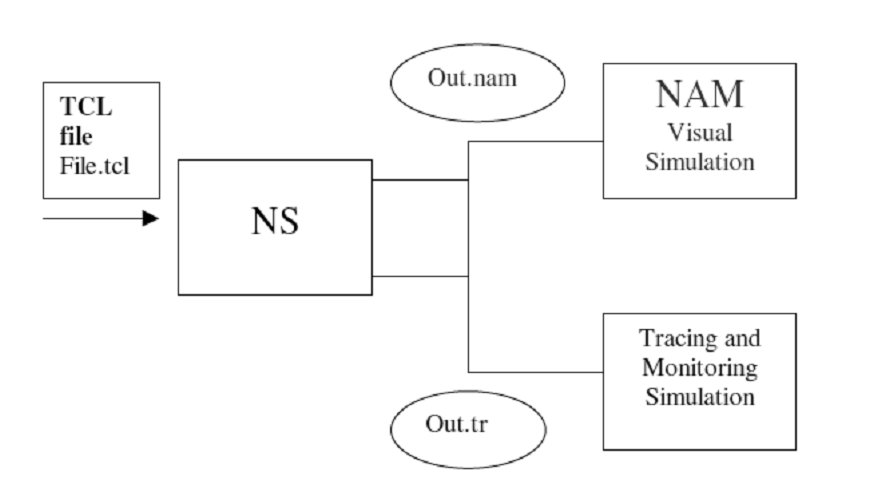
\includegraphics[scale=0.65]{nspic.PNG}
\caption{NS2 structure\label{overflow}}
\label{f5}
\end{figure}
\subsection{Awk Script}
The basic function of  awk  is to search files for lines (or other units of text) that 
contain certain patterns. When a line matches one of the patterns, awk  performs specified 
actions on that line. The awk  keeps processing input lines in  this way until the end of the input 
files are reached.


Programs in awk are different from programs in most other languages, because awk programs 
are data-driven; that is, we describe the data to work with, and then what to do when we find 
it. Most other languages are  procedural.  When working with procedural languages, it is 
usually much harder to clearly describe the data of our program will process. For this 
reason, awk programs are often refreshingly easy to both write and read.
When we run  awk, we can specify an  awk  program  that tells  awk  what to do. The program 
consists of a series of  rules. It may also contain  function definitions, an advanced feature 
which we will ignore for now. Each rule specifies one pattern to search for, and one action to 
perform when that pattern is found. 
\section{Experimental Setup}
Each topology is established using Network simulator 2. Eight different topology is implemented. In each topology the number of sensor nodes are same. There are 50 sensor nodes. Number of mobile sink in network changes from 1 to 8 in each topology. There is also base station in each topology. Modified clustering algorithm with mobile sink based data gathering applied in each topology. The simulation start time, end time, data transfer start time are similar to all topology.
The basic parameters of simulation are listed in  Table.\ref{table3}
\\
\begin{table*}[ht]
\centering
\renewcommand\arraystretch{2.4} \setlength\minrowclearance{2.4pt}
\caption{\label{table3} Simulation Parameters}
\vspace{5mm}
{
%\tiny\addtolength{\tabcolsep}{-7pt}
\hfill{}
\begin{tabular}{|p{0.3\linewidth}|p{0.3\linewidth}|}
%\begin{tabular}{|l|l|l|} 
  \hline
 \textbf{Name of Parameter } & \textbf{Value}  \\ 
 \hline
 Topography  & 1000*1000  \\ 
 \hline
 Protocol  & AODV  \\
 \hline
 Sensor Nodes & 50 \\  
 \hline
 Simulation Period  & 0.0 to 200.0 S\\ 
 \hline
 Size of ifq  & 100  \\ 
\hline
\end{tabular}}
\hfill{}
\end{table*}
\\
The nam output files of topology with different mobile sinks are given in appendices. After simulating each topology with varying number of mobile sinks the performance of each network evaluated using awk script. The parameters considered for performance analysis are average packet delivery ratio, Number of Dropped packets, Residual Energy, Sent-Received packet count. The values of performance parameters obtained from eight topology is given in Table \ref{table4}
\newpage
\begin{table*}[!ht]
\small
\renewcommand\arraystretch{2.4} \setlength\minrowclearance{2.4pt}
\centering
\caption{\label{table4} Result Analysis}
%\tiny\addtolength{\tabcolsep}{-7pt}
\hfill{}
\begin{tabular}{ |p{3.5cm}||p{1cm}|p{1cm}|p{1cm}|p{1cm}|p{1cm}|p{1cm}|p{1cm}|p{1cm}|}
 \hline
& \multicolumn{8}{|c|}{\textbf{NUMBER OF MOBILE SINKS}} \\
 \hline
\textbf{PARAMETERS} &1&2&3&4&5&6&7&8\\
 \hline
 Packets Sent   & 4772 &4805&4823&4818&4831&4808&4817&4805\\
 \hline
 Packets Received& 4736 &4769&4778&4765&4784&4763&4773&4763\\
 \hline
 Packet Dropped &36 &36&45&53&47&45&44&42\\
 \hline
 Packet Delivery Ratio  &99.25 &99.25&99.07&98.90&99.03&98.88&99.09&99.13\\
 \hline
 Normalised overhead& 0.75& 0.80&0.83&0.88&0.88&1.10&0.90&0.99\\
 \hline
 Routing overhead&  0.88& 0.94&0.97&1.03&1.03&1.28&1.06&1.16\\
 \hline
 Number of Mobile Sinks&1&2&3&4&5&6&7&8\\
 \hline
 Total Nodes(BS+MS+Sensor)&51&52&53&54&55&56&57&58\\
 \hline
  Residual Energy&92.653&92.94&93.22&92.690&92.56&92.825&92.416&92.299\\
 \hline
\end{tabular}\hfill{}
\end{table*}\\
Number of Packets sent and received measured and from analysis it is clear that MS3 has sent more packets. The packet sent versus received graph is shown in Figure.\ref{p1}


%\begin{figure[!ht]}
%\centering
%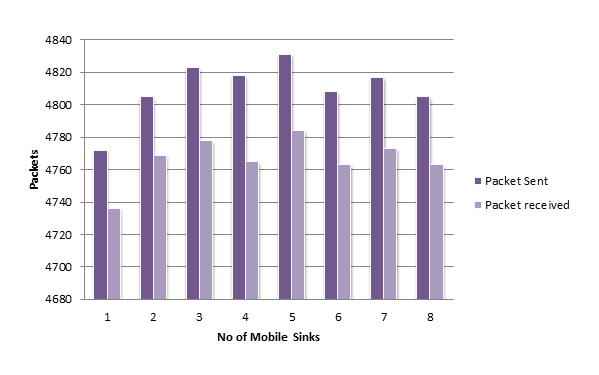
\includegraphics[scale=0.70]{PacketSentVsReceived.PNG}
%\caption{\label{p1} PacketSent Vs Received}
%\end{figure}\\
\begin{figure}
\center
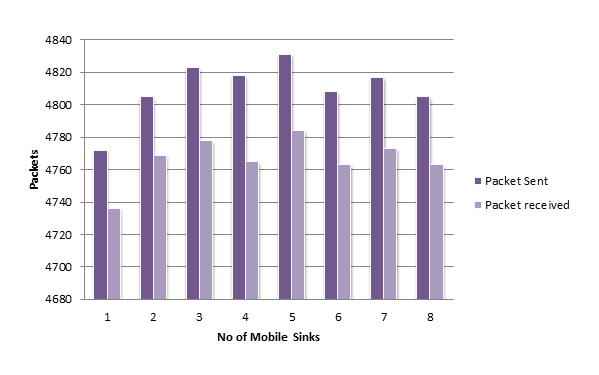
\includegraphics[scale=0.80]{PacketSentVsReceived.PNG}
\caption{PacketSent Vs Received}
\label{p1}
\end{figure}\\

The graph showing the number of packets dropped is given in Figure.\ref{p2}. From analysis graph it is clear that MS1 and MS2 have less number of dropped packets. Topology with 5 Mobile Sink have highest number of dropped packets.

\begin{figure}
\center
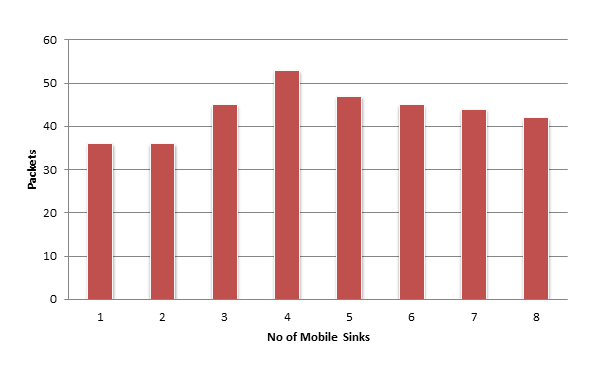
\includegraphics[scale=0.75]{PacketDropped.PNG}
\caption{Packet Dropped}
\label{p2}
\end{figure}
Packet delivery ratio is the ratio between the received packets by the destination and generated packets by source. Analysis based on Packet delivery ratio shows that MS1 and MS2 gives better performance. The analysis graph is shown in Figure.\ref{a1}.
\begin{figure}
\center
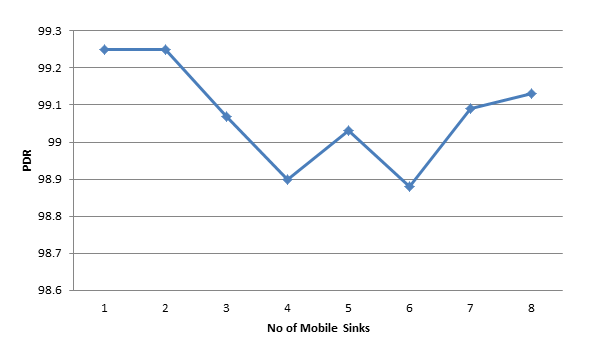
\includegraphics[scale=0.75]{PacketDeliveryRatio.PNG}
\caption{Packet Delivery Ratio}
\label{a1}
\end{figure}\\

Each node in topology have an initial value for energy at the starting of simulation. This is called initial energy. Due to packet transmission and reception every node losses particular amount of energy. Residual energy is termed as the current value of energy in a node after reception or transmission of packets. Analysis based on the residual energy of network shows that MS1 has high residual energy as compared to other topologies. The analysis graph based on residual energy shown in Figure.\ref{a2}.
\begin{figure}
\center
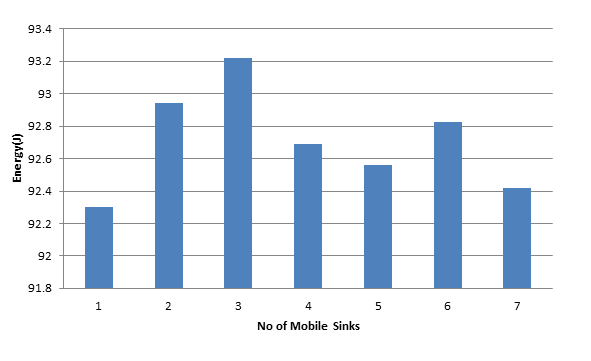
\includegraphics[scale=0.75]{ResidualEnergy.PNG}
\caption{Residual Energy}
\label{a2}
\end{figure}\\

The analysis based on total number of nodes(Total of sensor nodes, base station and mobile sink) used in each topology given in Figure.\ref{a3}. It is incremented as number of mobile sink increases. There is no change in the number of base station and sensor nodes required in each topology,only the number of mobile sink varies in each topology.
Figure.\ref{a3}
\begin{figure}
\center
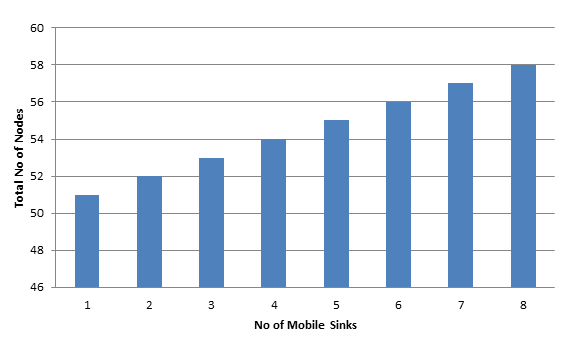
\includegraphics[scale=0.75]{totalnodes.PNG}
\caption{Total number of Nodes}
\label{a3}
\end{figure}\\

From analysis it is clear that topology with one and two mobile sink give better performance. That is when network with 50 dynamic sensor nodes are used for data gathering, one or two mobile sink can give better performance in terms of Residual energy, Packet delivery ratio, Number of dropped packets. Major advantage of proposed system is the consideration of dynamic environment. This analysis help to avoid the problem of finding mobile sink required for data gathering in wireless sensor networks.

Major advantage of the proposed system is the application of modified clustering algorithm for data gathering. It allow the cluster head selection and clustering algorithm in the dynamic environment. The proposed system reduce the burden of mobile sink number estimation for a particular network and in effect increases the performance and reduces the cost.
\section{Findings}
From the analysis it is found that for a network with \textbf{50} dynamic sensor nodes only \textbf{1} mobile Sink is required to gather data with high performance
\pagebreak
\clearpage
\chapter{CONCLUSION AND FUTURE SCOPE}
\label {conc}
Studied the energy consumption problem of wireless sensor network in Big data gathering. Mobile sink approach can solve this problem of energy consumption. Heterogeneous environment is used for clustering and clustering method relies up on the power of nodes. For data gathering two sink approach is proposed. Static sink and mobile sink are used to gather data. Performance analysis conducted to find out optimum number of mobile sink for a given sensor network. This analysis avoid the resource under utilization and over utilization with out knowing the required number of mobile sink for a particular network.


Securing the critical data while gathering is an important task since so many vulnerabilities and attacks are there in dynamic environment. Certificate less-effective key management (CL-EKM) protocol can be  for secure communication in dynamic WSNs. CL-EKM method already applied in dynamic environment. But when it comes to sensor network with mobile sink approach CL-EKM is an open problem to be solved. 
\pagebreak
\pagestyle{empty}
\begin{singlespace}
  %\bibliography{refs}
  \addcontentsline{toc}{chapter}{REFERENCES}
  \begin{thebibliography}{1}
\bibitem{}
Daisuke Takaishi, Hiroki Nishiyama,Nei Kato, and Ryu Miura,\textit{"Towards Energy Efficient Big Data Gathering in Densely Distributed Sensor Networks"}, IEEE Transactions on Emerging Topics in Cloud Computing, February 2014
\bibitem{}
Yi Sun, Can Cui, Shanshan Ke, Jun Lu, \textit{"Research on Dynamic Clustering Routing Considering 
Node Load for Wireless Sensor Networks"}, Communications and Network, 2013, 5, 508-511
\bibitem{}
Prashant Krishnan, \textit{"Comparison and Performance Analysis of Dynamic 
and Static Clustering Based Routing Scheme in 
Wireless Sensor Network"}, International Journal of Advanced Research in Computer and Communication Engineering Vol. 2, Issue 4, April 2013
\bibitem{}
Said Benkirane, Abderrahim Beni hssane, Moulay Lahcen Hasnaoui, Mostafa Saadi and Mohamed Laghdir,\textit{"Weighted Dynamic Distributed Clustering 
Protocol For Heterogeneous Wireless 
Sensor Network
"}, International Journal of Wireless and Mobile Networks(IJWMN) Vol. 4, No. 6, December 2012

\bibitem{}
Deepali Virmani, Akshay Jain, Ankit Khandelwal, Divik Gupta, Nitin Garg, \textit{"Dynamic Clustering Protocol for Data Forwarding in 
Wireless Sensor Networks
"}, International Journal of Computers and Technology, 2013
\bibitem{}
Lin Zhao, Zhibo Chen, Guodong Sun, \textit{"Dynamic Cluster-based Routing for Wireless
Sensor Networks"}, Journal Of Networks, Vol. 9, No. 11, November 2014.
\bibitem{}
Tal Anker, Danny Bickson, Danny Dolev and Bracha Hod, \textit{"Efficient Clustering for Improving Network Performance in Wireless Sensor Networks"}, EWSN'08 Proceedings of the 5th European conference on Wireless sensor networks, 2008
\bibitem{}
P. Sasikumar, Sibaram Khara \textit{"K-Means Clustering In Wireless Sensor Networks"}, International Conference on Computational Intelligence and Communication Networks, 2012
\bibitem{}
A.B.M.Alim Al Islam, Chowdhury Sayeed Hyder, Humayun Kabir, Mahmuda Naznin, \textit{"Stable Sensor Network (SSN): A Dynamic Clustering 
Technique for Maximizing Stability in Wireless 
Sensor Networks"}, Wireless Sensor Network, 2010, 2, 538-554 .
\bibitem{}
Rashmi KR, Shivakumar AB, Ananda Babu J, \textit{"Energy Efficient Clustering Techniques 
For Mobile Data Gathering In Distributed 
WSN
"}, International Journal of Advanced Technology in Engineering and Science
Volume No 03, Special Issue No. 01, March 2015 
\bibitem{}
Enrique J. Duarte-Melo, Mingyan Liu, \textit{"Data-gathering wireless sensor networks: organization
and capacity"}, Elsevier, Computer Networks 43 (2003)519-537 
\bibitem{}
Vijayalaxmi, \textit{"An Efficient way to Gather Big Data in WSN 
using Mobile Sink Routing"}, International Journal of Advanced Research in Computer and Communication Engineering, Vol. 4, Issue 8, August 2015
\bibitem{}
Seref Sagiroglu and Duygu Sinanc,\textit{"BigData:A Review"}, in Proc.Int.Conf.CTS,2013
\bibitem{}
Javier Andreu-Perez, Carmen C. Y. Poon, Robert D. Merrifield, Stephen T. C. Wong,
and Guang-Zhong Yang \textit{"Big Data for Health"}, Ieee Journal Of Biomedical And Health Informatics, Vol. 19, No. 4, July 2015
\bibitem{}
Lidice Garcia Rios, Jose Alberto Incera Diguez \textit{"Big Data Infrastructure for analyzing data generated by Wireless Sensor Networks"}, IEEE International Congress on Big Data, 2014 
\bibitem{}
Stephen Kaisler, Frank Armour, J. Albert Espinosa \textit{"Introduction to Big Data: Challenges, Opportunities and Realities "}, 47th Hawaii International Conference on System Science, 2014
\end{thebibliography}
\end{singlespace}

%\newpage
%\begin{center}
%\textbf{\Large PUBLICATIONS}
%\end{center}

%\begin{description}
%\item[{[1]}]Antu Raj S, Sangeetha Jose\textit{"Study On Cognitive Wireless Mesh Networks For Emergency And Public Safety Situations"}, GECIAN National Conference, September 2015, Pages 25-29
%\end{description}


%\begin{appendices}
\appendix
%\addcontentsline{toc}{chapter}{Appendix}
\addtocontents{toc}{\protect\contentsline{chapter}{APPENDIX}{}}
  \chapter{Screenshots}
 % \chapter{Mauris euismod}
\begin{figure}[ht!]
\centering
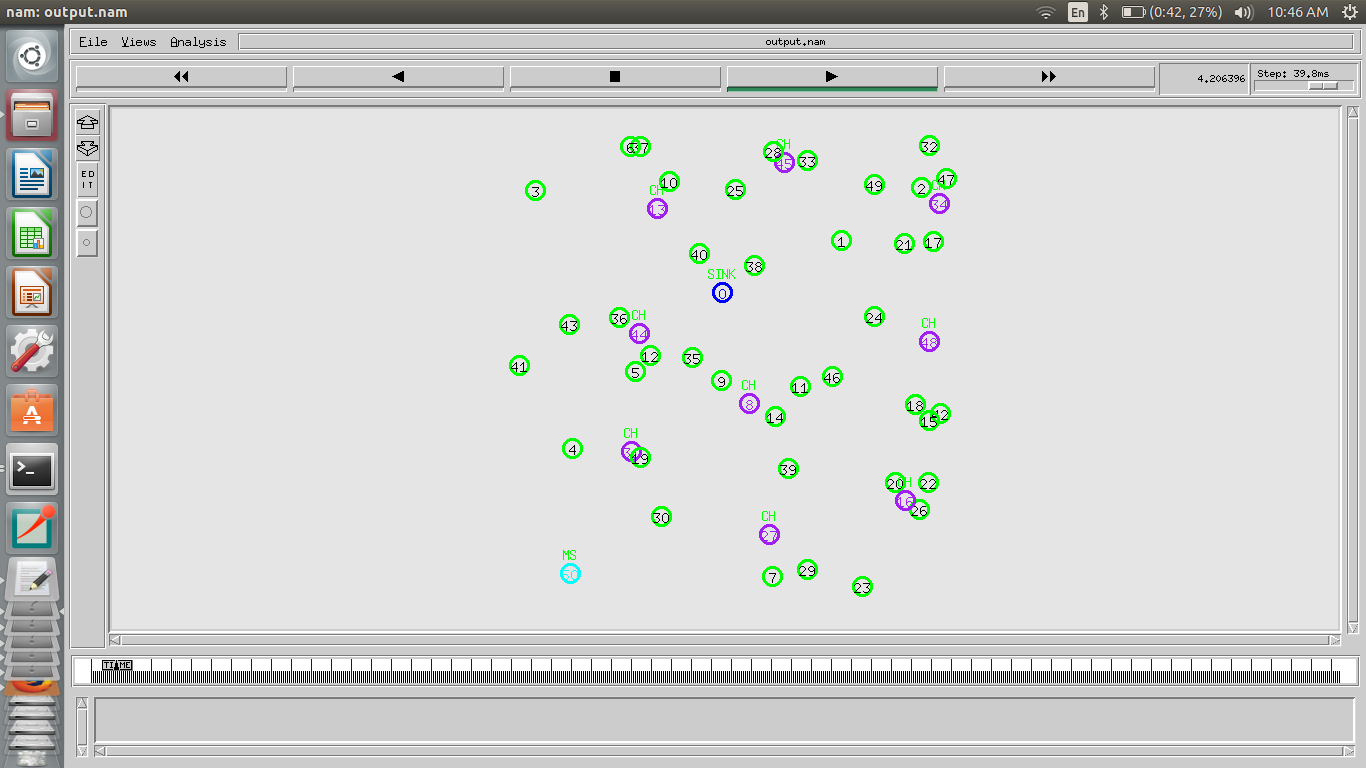
\includegraphics[scale=0.25]{output1sink.PNG}
\caption{NAM output of topology with 1 mobile sinks\label{overflow}}
\label{f6}
\end{figure}
\begin{figure}[h]
\centering
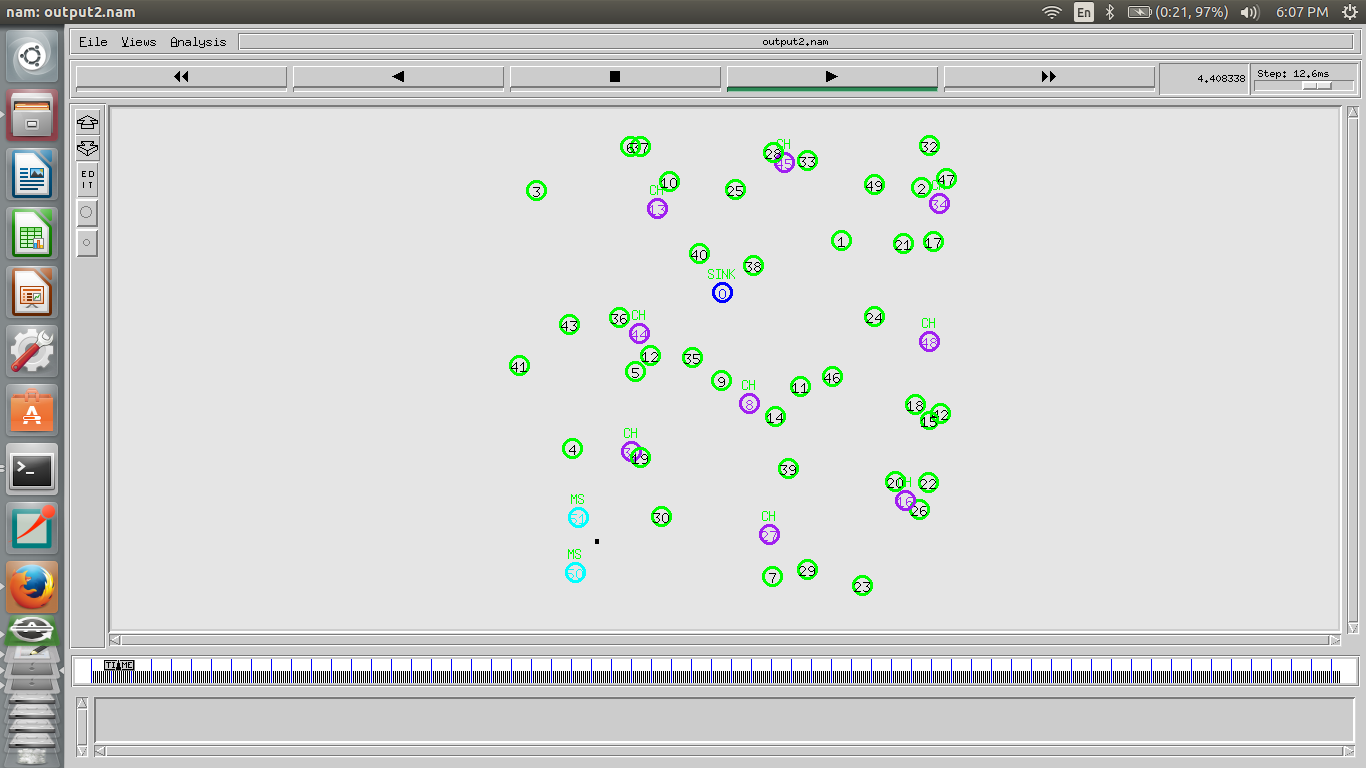
\includegraphics[scale=0.25]{output2sink.PNG}
\caption{NAM output of topology with 2 mobile sinks\label{overflow}}
\label{f7}
\end{figure}


\pagebreak
\newgeometry{left=1.5in,right=1in,top=1in,bottom=1.9in}
\pagestyle{fancy}
\lhead{}
\rhead{\textit{Analysis of Mobile Sink Based Big Data Gathering in DWSNs}}
\lfoot{\textit{Department of Information Technology}}
\rfoot{\textit{GECI}}
\cfoot{\thepage}
\renewcommand{\footrulewidth}{1pt}
\renewcommand{\headrulewidth}{1pt}
\setlength{\headsep}{0.5in}
\begin{figure}[ht!]
\centering
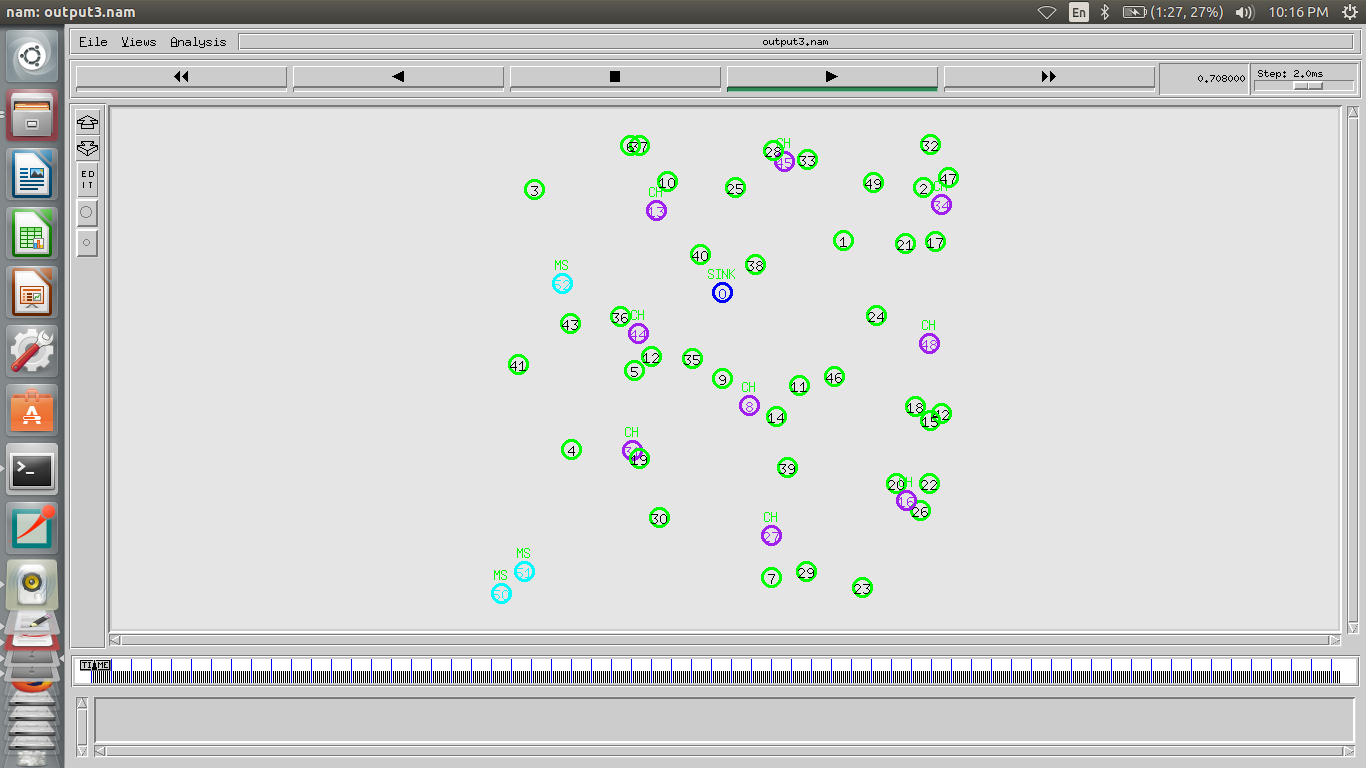
\includegraphics[scale=0.25]{3sink.PNG}
\caption{NAM output of topology with 3 mobile sinks\label{overflow}}
\label{f8}
\end{figure}
\begin{figure}[h]
\centering
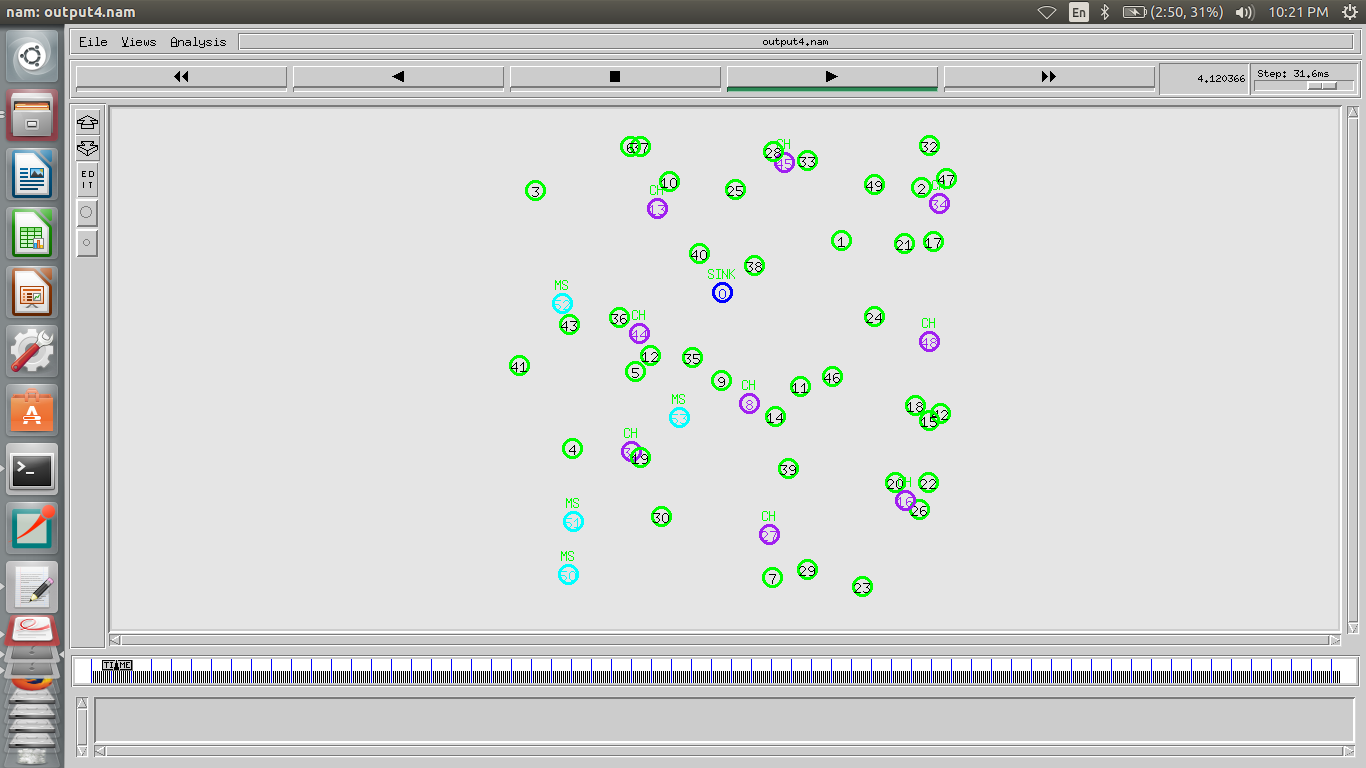
\includegraphics[scale=0.25]{4sink.PNG}
\caption{NAM output of topology with 4 mobile sinks\label{overflow}}
\label{f9}
\end{figure}
\begin{figure}[ht!]
\centering
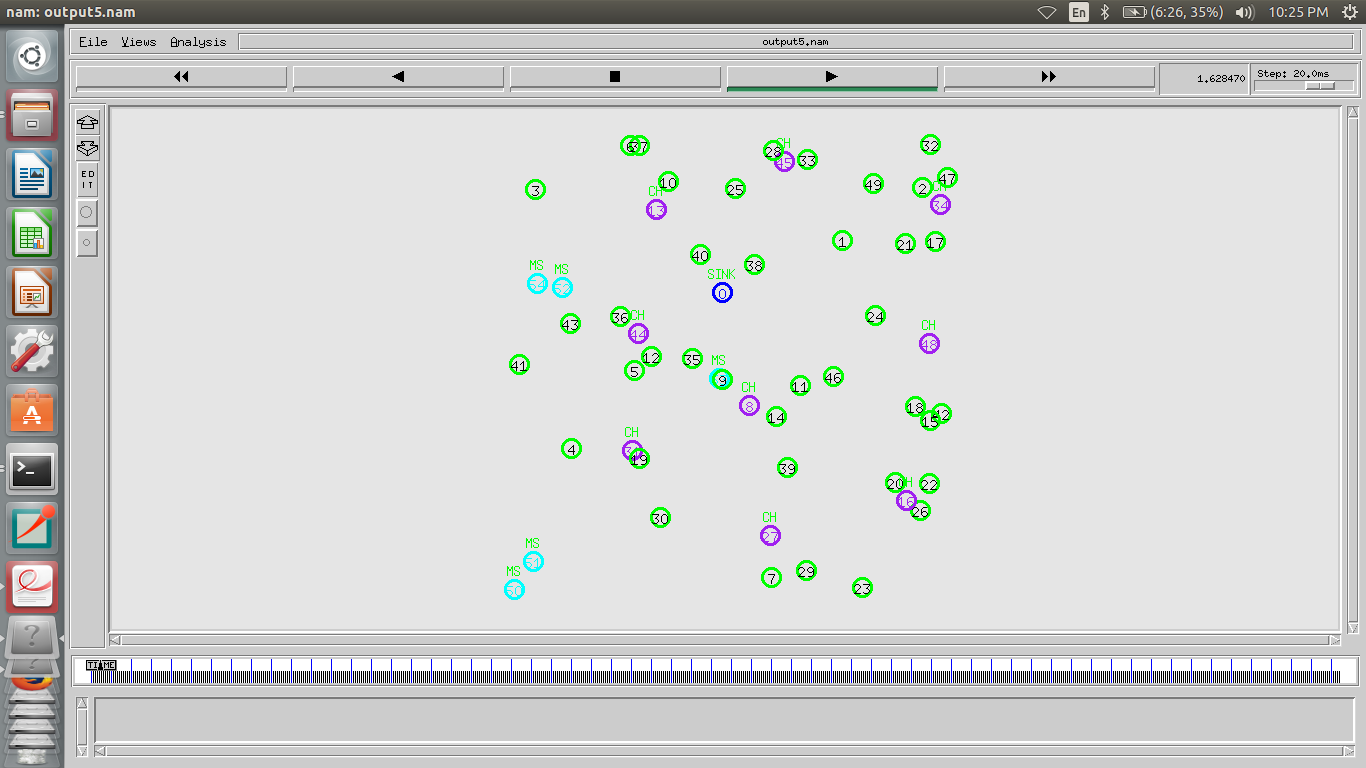
\includegraphics[scale=0.25]{5sink.PNG}
\caption{NAM output of topology with 5 mobile sinks\label{overflow}}
\label{f10}
\end{figure}
\begin{figure}[h]
\centering
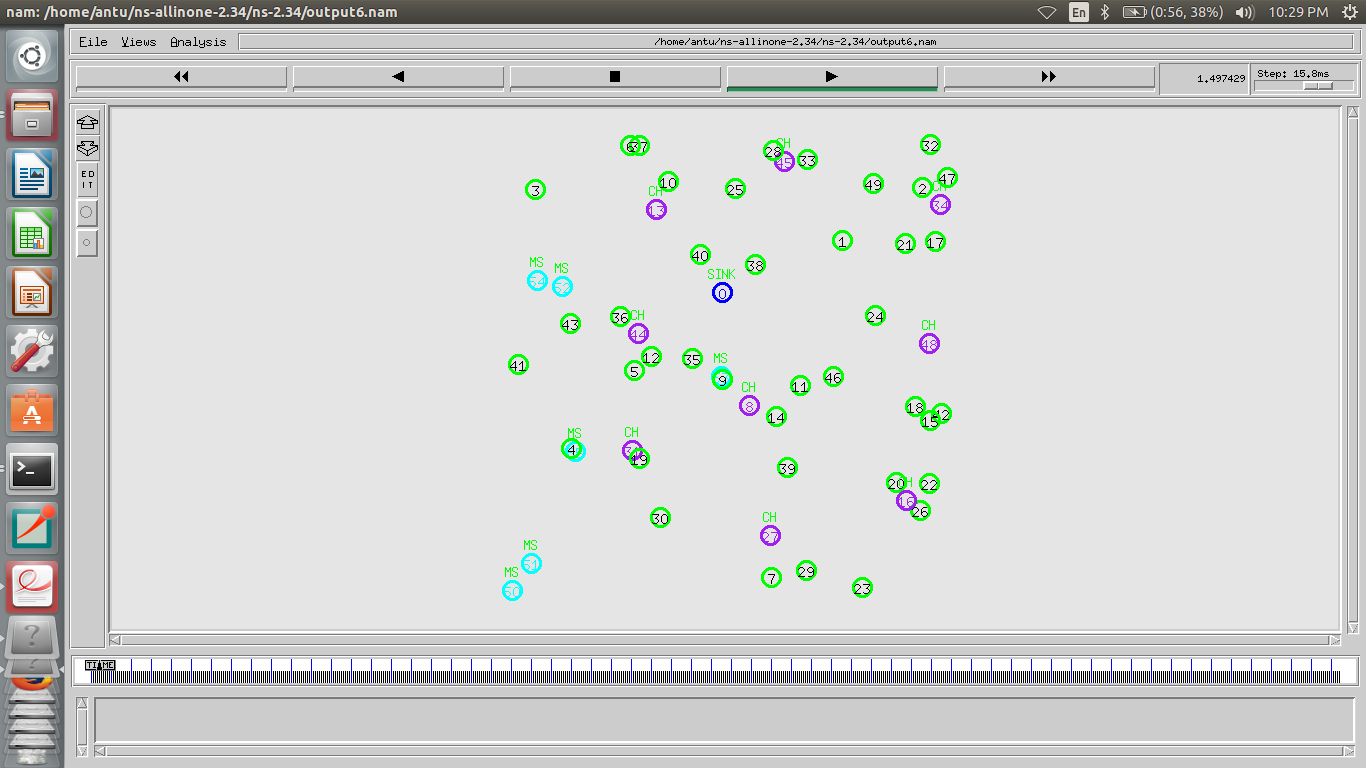
\includegraphics[scale=0.25]{6sink.PNG}
\caption{NAM output of topology with 6 mobile sinks\label{overflow}}
\label{f11}
\end{figure}
\begin{figure}[ht!]
\centering
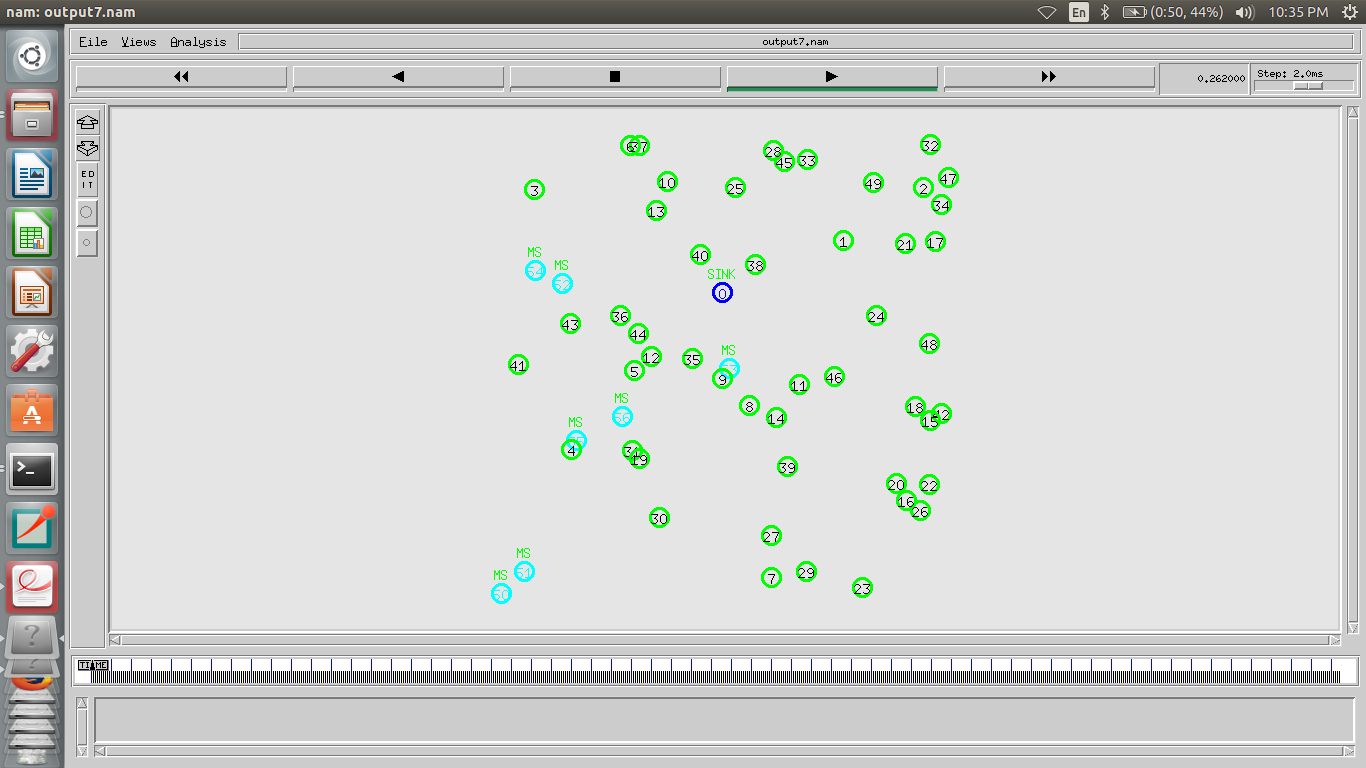
\includegraphics[scale=0.25]{7sink.PNG}
\caption{NAM output of topology with 7 mobile sinks\label{overflow}}
\label{f12}
\end{figure}
\begin{figure}[h]
\centering
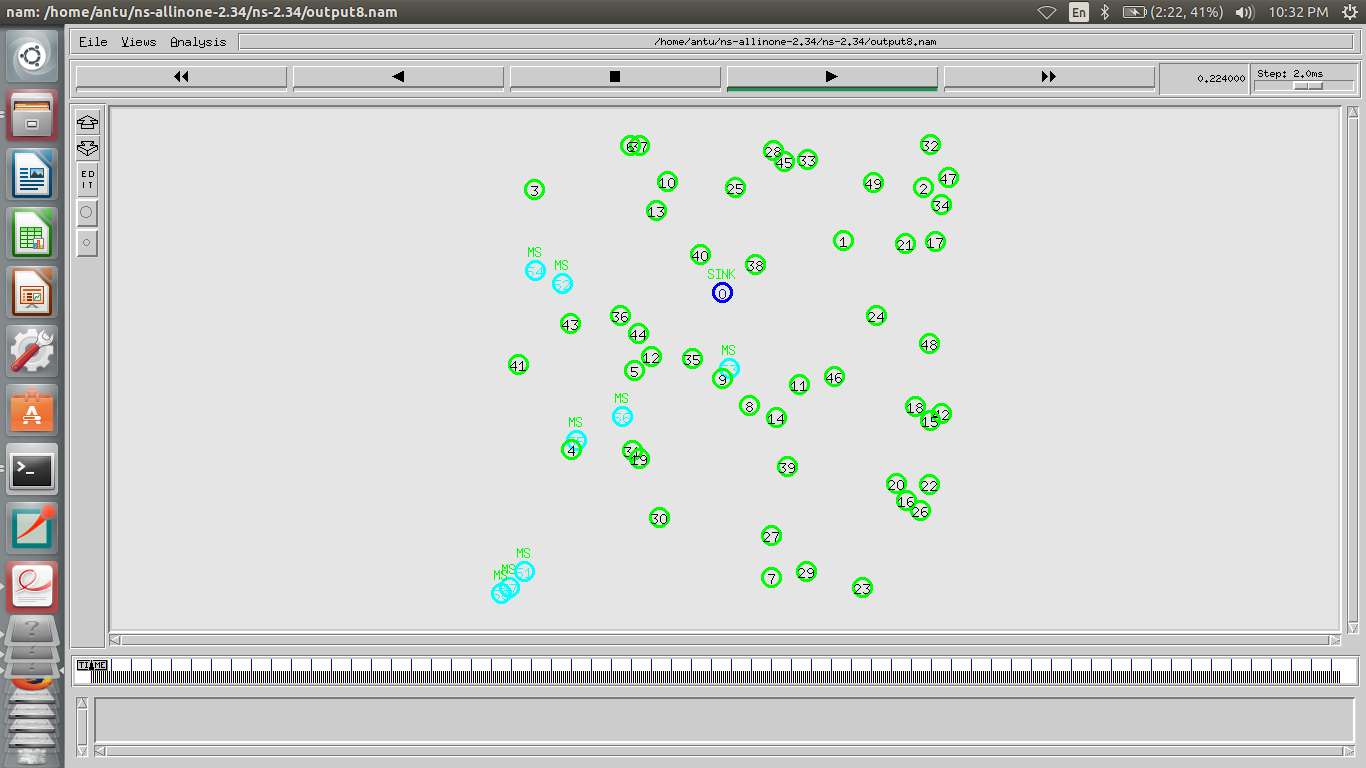
\includegraphics[scale=0.25]{8sink.PNG}
\caption{NAM output of topology with 8 mobile sinks\label{overflow}}
\label{f13}
\end{figure}
%\addtocontents{toc}{\protect\contentsline{chapter}{PUBLICATIONS}{}}
  \chapter{Publications}  
\begin{description}
\item[{[1]}]Antu Raj S, Sangeetha Jose\textit{"A New Approach for Big Data Gathering In Dynamic Wireless Sensor Networks"}, International Journal of Science and Research, ISSN 2319-7064, Volume 5 Issue 3, March 2016 [Communicated]
\item[{[2]}]Antu Raj S, Sangeetha Jose\textit{"Study On Cognitive Wireless Mesh Networks For Emergency And Public Safety Situations"}, GECIAN National Conference, September 2015, Pages 25-29
\end{description}

%\end{appendices}
\end{document}